\documentclass[12pt, a4paper]{article}
\usepackage{mathptmx} % Times New Roman font
\usepackage[utf8]{inputenc}
\usepackage[T1]{fontenc}
\usepackage{geometry}
\usepackage{titlesec}
\usepackage{hyperref}
\usepackage{graphicx}
\usepackage{float}
\usepackage{tocloft}
\usepackage{amsmath,amsfonts,amssymb}
\usepackage{tikz}
\usetikzlibrary{shapes,arrows,positioning,calc,decorations.pathreplacing}
\usepackage{listings}
\usepackage{xcolor}
\usepackage{booktabs}
\usepackage{tabularx}
\usepackage{multirow}
\usepackage{array}
\usepackage{caption}
\usepackage{subcaption}
\usepackage{enumitem}
\usepackage{fancyhdr}

\geometry{margin=1in}
\setlength{\cftbeforesecskip}{1.5em}
\setlength{\cftsecnumwidth}{2em}

% Code listing style
\lstdefinestyle{python}{
    backgroundcolor=\color{gray!10},
    basicstyle=\ttfamily\footnotesize,
    breaklines=true,
    commentstyle=\color{green!60!black},
    keywordstyle=\color{blue},
    stringstyle=\color{orange!80!black},
    numbers=left,
    numberstyle=\tiny\color{gray},
    numbersep=5pt,
    frame=single,
    framesep=5pt,
    language=Python
}

\hypersetup{
    colorlinks=true,
    linkcolor=blue,
    filecolor=magenta,
    urlcolor=cyan,
}

% Page header/footer
\pagestyle{fancy}
\fancyhf{}
\rhead{COMP6826001 - Deep Learning}
\lhead{Doodle Recognition Project}
\cfoot{\thepage}

\begin{document}

% ============================================================================
% TITLE PAGE
% ============================================================================
\begin{titlepage}
    \centering
    \vspace*{0.5cm}
    
    \includegraphics[width=0.5\textwidth]{../proposal-dl/binuslogo.png}
    
    \vspace{1cm}
    
    {\Large \textbf{BINUS University} \par}
    \vspace{0.3cm}
    {\large School of Computer Science \par}
    {\large Computer Science Department \par}
    
    \vspace{1.5cm}
    
    {\LARGE \textbf{FINAL PROJECT REPORT} \par}
    \vspace{0.5cm}
    {\Large COMP6826001 - Deep Learning \par}
    
    \vspace{1.5cm}
    
    {\Huge \textbf{Gamified Doodle Recognition for English Vocabulary Acquisition using Deep Learning} \par}
    
    \vspace{2cm}
    
    {\large \textbf{Team Members:} \par}
    \vspace{0.5cm}
    \begin{tabular}{ll}
        \textbf{Valent Nathanael} & 2702343706 \\
        \textbf{Joceline Araki} & 2702338334 \\
        \textbf{Lauw, Samuel Lelono} & 2702348026 \\
    \end{tabular}
    
    \vspace{1.5cm}
    
    {\large Class: All Class \par}
    \vspace{0.3cm}
    {\large Academic Year: 2025/2026 \par}
    {\large Term: Odd \par}
    
    \vfill
    
    {\large Campus: Kemanggisan / Alam Sutera \par}
\end{titlepage}

% ============================================================================
% TABLE OF CONTENTS
% ============================================================================
\renewcommand{\cfttoctitlefont}{\hfill\Large\bfseries}
\renewcommand{\cftaftertoctitle}{\hfill}
\tableofcontents
\newpage

% ============================================================================
% ABSTRACT
% ============================================================================
\section*{Abstract}
\addcontentsline{toc}{section}{Abstract}

This project presents a comprehensive deep learning solution for real-time doodle recognition, designed to facilitate English vocabulary acquisition for Indonesian learners through gamification. We developed and evaluated multiple deep learning architectures including ResNet18 (transfer learning) and traditional computer vision approaches using OpenCV similarity matching.

Our ResNet18 model achieves \textbf{75.03\% top-1 accuracy} and \textbf{90.70\% top-3 accuracy} across 340 doodle categories from the QuickDraw dataset, containing over 1 million training samples.

The final application is deployed as a Flask-based web interface with real-time inference, featuring both free-draw mode for exploration and a gamified challenge mode with scoring mechanics. The system processes drawings in real-time (400ms intervals) and provides instant visual feedback, making it suitable for educational deployment targeting English vocabulary learning in Indonesia.

\textbf{Keywords:} Deep Learning, Doodle Recognition, Transfer Learning, ResNet, QuickDraw Dataset, Educational Technology

\newpage

% ============================================================================
% 1. INTRODUCTION
% ============================================================================
\section{Introduction}

\subsection{Background}

English proficiency is a critical skill in Indonesia's educational landscape, with the language serving as a key differentiator in academic and professional contexts. However, traditional rote memorization of vocabulary can be disengaging for young learners, leading to poor retention and lack of motivation.

Hand-drawn sketch recognition has emerged as a compelling application of deep learning, combining computer vision with human-computer interaction. Google's Quick, Draw! experiment demonstrated that neural networks can recognize hand-drawn doodles in real-time, even when drawings are abstract or incomplete. This technology presents an opportunity to transform language learning into an engaging, interactive experience.

The intersection of deep learning and educational technology offers a unique opportunity to address both technical and pedagogical challenges. By leveraging state-of-the-art neural network architectures for image classification, we can create systems that understand the inherent variability in human drawings while providing immediate feedback that reinforces learning.

\subsection{Problem Statement}

Despite advancements in deep learning for image recognition, several challenges remain for doodle classification:

\begin{enumerate}
    \item \textbf{High Intra-class Variability}: Doodles of the same object can vary significantly between individuals in terms of style, abstraction level, and drawing skill.
    
    \item \textbf{Large Number of Categories}: The QuickDraw dataset contains 340 categories, making accurate classification challenging compared to standard benchmarks.
    
    \item \textbf{Incomplete and Abstract Drawings}: Unlike photographs, doodles are often incomplete, simplified, or abstract representations of objects.
    
    \item \textbf{Real-time Requirements}: Educational applications require fast inference to maintain user engagement and provide instant feedback.
    
    \item \textbf{Generalization to Children's Drawings}: Models trained on adult-drawn sketches may not generalize well to children's drawings, which often exhibit different characteristics.
\end{enumerate}

\subsection{Objectives}

The primary objectives of this project are:

\begin{enumerate}
    \item \textbf{Develop and Compare Multiple Deep Learning Models}: Implement and evaluate ResNet-based transfer learning and traditional OpenCV similarity matching approaches.
    
    \item \textbf{Achieve High Classification Accuracy}: Target top-1 accuracy above 70\% and top-3 accuracy above 85\% across all 340 categories.
    
    \item \textbf{Build a Real-time Web Application}: Create a Flask-based interface with sub-second inference and smooth user experience.
    
    \item \textbf{Implement Gamification Features}: Design challenge mode with scoring mechanics to enhance engagement and learning outcomes.
    
    \item \textbf{Evaluate Model Robustness}: Analyze model performance across different drawing styles and difficulty levels.
\end{enumerate}

\subsection{Significance}

This project contributes to both the technical and educational domains:

\begin{itemize}
    \item \textbf{Technical Contribution}: Comprehensive comparison of transfer learning and traditional CV approaches for sketch recognition.
    
    \item \textbf{Educational Impact}: A deployable tool for English vocabulary acquisition that combines visual-motor learning with immediate feedback.
    
    \item \textbf{Research Value}: Insights into the generalization capabilities of deep learning models on abstract, hand-drawn inputs.
    
    \item \textbf{Practical Application}: A complete end-to-end system from model training to web deployment suitable for classroom use.
\end{itemize}

\newpage

% ============================================================================
% 2. RELATED WORK
% ============================================================================
\section{Related Work}

\subsection{QuickDraw Dataset and Recognition}

The QuickDraw dataset, released by Google in 2017, contains over 50 million drawings across 345 categories, collected through the ``Quick, Draw!'' game. Each drawing is stored as timestamped stroke data, capturing the sequential nature of human sketching. Previous works have achieved varying levels of accuracy on this dataset:

\begin{itemize}
    \item \textbf{Ha \& Eck (2018)} demonstrated that recurrent neural networks (RNNs) can leverage stroke sequence information, achieving 75.4\% top-1 accuracy using a sketch-RNN architecture \cite{ha2017neural}.
    
    \item \textbf{Yu et al. (2017)} achieved 77.95\% accuracy using a multi-scale CNN ensemble on rendered bitmap images \cite{yu2017sketch}.
    
    \item \textbf{Google's Baseline CNN} reported 73.4\% accuracy using a simple convolutional architecture trained on bitmap representations.
\end{itemize}

\subsection{Transfer Learning for Image Classification}

Transfer learning has revolutionized image classification by enabling models trained on large datasets (ImageNet) to be fine-tuned for specific tasks:

\begin{itemize}
    \item \textbf{He et al. (2016)} introduced ResNet, demonstrating that residual connections enable training of very deep networks (50-152 layers) with improved performance \cite{he2016deep}.
    
    \item \textbf{Tan \& Le (2019)} proposed EfficientNet, achieving state-of-the-art accuracy with compound scaling of depth, width, and resolution \cite{tan2019efficientnet}.
    
    \item Transfer learning from ImageNet has been shown to improve performance even on domains significantly different from natural images, including medical imaging and satellite imagery.
\end{itemize}

\subsection{Traditional Computer Vision Approaches}

Traditional computer vision methods provide interpretable baselines for image recognition:

\begin{itemize}
    \item \textbf{Template Matching}: Direct pixel-level comparison using normalized cross-correlation.
    
    \item \textbf{Feature Matching}: Keypoint detection and descriptor matching using SIFT/ORB algorithms.
    
    \item \textbf{Histogram Comparison}: Statistical distribution matching for image similarity.
\end{itemize}

\subsection{Educational Technology and Gamification}

Research in educational technology has demonstrated the effectiveness of gamification:

\begin{itemize}
    \item \textbf{Deterding et al. (2011)} defined gamification as the use of game design elements in non-game contexts, identifying key mechanics that enhance engagement.
    
    \item \textbf{Vocabulary acquisition research} shows that multimodal learning (combining visual, auditory, and kinesthetic elements) improves retention compared to text-only approaches.
    
    \item \textbf{Immediate feedback} has been shown to be critical for language learning, enabling rapid error correction and reinforcement.
\end{itemize}

\newpage

% ============================================================================
% 3. METHODOLOGY
% ============================================================================
\section{Methodology}

\subsection{Dataset Description}

We utilized the QuickDraw dataset with the following characteristics:

\begin{table}[H]
\centering
\caption{Dataset Overview}
\begin{tabular}{ll}
\toprule
\textbf{Attribute} & \textbf{Value} \\
\midrule
Number of Categories & 340 \\
Images per Category & 3,000 \\
Total Images & 1,020,000 \\
Image Format & PNG (bitmap) \\
Original Size & 28×28 pixels \\
Processed Size & 160×160 pixels (ResNet) \\
Train/Val/Test Split & 70\% / 15\% / 15\% \\
\bottomrule
\end{tabular}
\end{table}

\textbf{Category Examples:} airplane, apple, banana, basketball, bear, bicycle, bird, book, butterfly, cake, car, cat, chair, clock, cloud, coffee cup, dog, door, eye, face, fish, flower, guitar, hammer, hat, house, key, leaf, moon, mountain, mushroom, pants, pencil, piano, pizza, rainbow, scissors, shoe, smile, snowflake, star, sun, table, telephone, tree, umbrella, violin, wheel, and 292 more categories.

\subsection{Data Preprocessing}

\subsubsection{Image Preprocessing Pipeline}

\begin{enumerate}
    \item \textbf{Resize}: Images resized to target dimensions (160×160 for ResNet)
    \item \textbf{Grayscale to RGB}: Converted single-channel to 3-channel for transfer learning compatibility
    \item \textbf{Polarity Normalization}: Ensured consistent dark strokes on light background
    \item \textbf{Normalization}: Applied ImageNet statistics for transfer learning models
\end{enumerate}

\subsubsection{Data Augmentation (Training Only)}

\begin{lstlisting}[style=python, caption=Data Augmentation Transforms]
train_transform = transforms.Compose([
    transforms.RandomCrop(160, padding=8),
    transforms.RandomHorizontalFlip(p=0.5),
    transforms.RandomRotation(15),
    transforms.RandomAffine(
        degrees=0, translate=(0.1, 0.1),
        scale=(0.9, 1.1), shear=5
    ),
    transforms.ColorJitter(
        brightness=0.2, contrast=0.2
    ),
    transforms.ToTensor(),
    transforms.Normalize(
        mean=[0.5, 0.5, 0.5],
        std=[0.5, 0.5, 0.5]
    )
])
\end{lstlisting}

\subsection{Model Architecture 1: ResNet18 with Transfer Learning}

\subsubsection{Architecture Overview}

We employed ResNet18 pre-trained on ImageNet (1.2M images, 1000 classes) and modified the classifier head for 340-class doodle classification:

\begin{figure}[H]
\centering
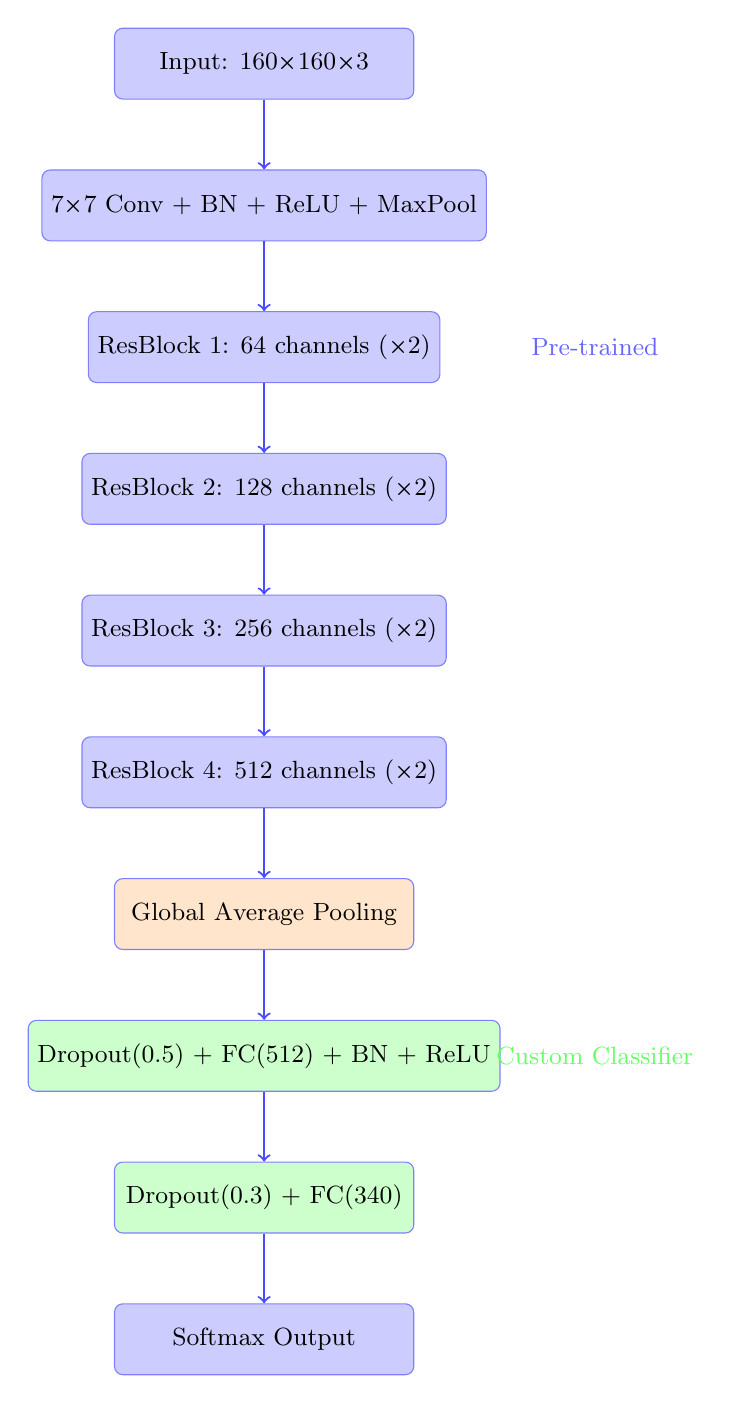
\begin{tikzpicture}[
    node distance=1.8cm,
    block/.style={rectangle, draw=blue!50, fill=blue!20, minimum width=3.8cm, minimum height=0.9cm, text centered, font=\small, rounded corners=3pt},
    arrow/.style={->, thick, color=blue!70}
]

\node[block] (input) {Input: 160×160×3};
\node[block, below of=input] (conv1) {7×7 Conv + BN + ReLU + MaxPool};
\node[block, below of=conv1] (res1) {ResBlock 1: 64 channels (×2)};
\node[block, below of=res1] (res2) {ResBlock 2: 128 channels (×2)};
\node[block, below of=res2] (res3) {ResBlock 3: 256 channels (×2)};
\node[block, below of=res3] (res4) {ResBlock 4: 512 channels (×2)};
\node[block, below of=res4, fill=orange!20] (gap) {Global Average Pooling};
\node[block, below of=gap, fill=green!20] (fc1) {Dropout(0.5) + FC(512) + BN + ReLU};
\node[block, below of=fc1, fill=green!20] (fc2) {Dropout(0.3) + FC(340)};
\node[block, below of=fc2] (output) {Softmax Output};

\draw[arrow] (input) -- (conv1);
\draw[arrow] (conv1) -- (res1);
\draw[arrow] (res1) -- (res2);
\draw[arrow] (res2) -- (res3);
\draw[arrow] (res3) -- (res4);
\draw[arrow] (res4) -- (gap);
\draw[arrow] (gap) -- (fc1);
\draw[arrow] (fc1) -- (fc2);
\draw[arrow] (fc2) -- (output);

\node[right of=res1, node distance=4.2cm, text=blue!60, font=\small] {Pre-trained};
\node[right of=fc1, node distance=4.2cm, text=green!60, font=\small] {Custom Classifier};

\end{tikzpicture}
\caption{ResNet18 Architecture for Doodle Classification}
\end{figure}

\subsubsection{Custom Classifier Head}

\begin{lstlisting}[style=python, caption=Custom Classifier Architecture]
model.fc = nn.Sequential(
    nn.Dropout(0.5),
    nn.Linear(512, 512),
    nn.BatchNorm1d(512),
    nn.ReLU(inplace=True),
    nn.Dropout(0.3),
    nn.Linear(512, num_classes)  # 340 classes
)
\end{lstlisting}

\subsubsection{Two-Stage Training Strategy}

\begin{enumerate}
    \item \textbf{Stage 1 (Epochs 1-10)}: Freeze ResNet backbone, train only classifier
    \begin{itemize}
        \item Learning rate: 1e-3
        \item Purpose: Stabilize classifier with pre-trained features
        \item Trainable parameters: 438,100
    \end{itemize}
    
    \item \textbf{Stage 2 (Epochs 11-40)}: Unfreeze all parameters, fine-tune entire network
    \begin{itemize}
        \item Backbone learning rate: 1e-4
        \item Classifier learning rate: 5e-4
        \item Purpose: Adapt features to doodle-specific patterns
        \item Total parameters: 11,614,612
    \end{itemize}
\end{enumerate}

\subsection{Model Architecture 2: OpenCV Similarity Matching}

As a baseline comparison, we implemented a traditional computer vision approach using OpenCV:

\subsubsection{Multi-Method Similarity}

\begin{enumerate}
    \item \textbf{Template Matching}: Normalized cross-correlation (TM\_CCOEFF\_NORMED)
    \item \textbf{Feature Matching}: SIFT/ORB keypoint detection and descriptor matching
    \item \textbf{Histogram Comparison}: Correlation, intersection, and Bhattacharyya distance
\end{enumerate}

\begin{equation}
    \text{Similarity}_{\text{final}} = \frac{1}{3}\left(S_{\text{template}} + S_{\text{features}} + S_{\text{histogram}}\right)
\end{equation}

\subsection{Evaluation Metrics}

\begin{itemize}
    \item \textbf{Top-1 Accuracy}: Percentage of correctly classified samples
    \item \textbf{Top-3 Accuracy}: Percentage where correct label is in top 3 predictions
    \item \textbf{Top-5 Accuracy}: Percentage where correct label is in top 5 predictions
    \item \textbf{Confusion Matrix}: Per-class performance analysis
    \item \textbf{Inference Time}: Time per prediction for real-time requirements
\end{itemize}

\newpage

% ============================================================================
% 4. IMPLEMENTATION & RESULTS
% ============================================================================
\section{Implementation \& Results}

\subsection{Development Environment}

\begin{table}[H]
\centering
\caption{Development Environment}
\begin{tabular}{ll}
\toprule
\textbf{Component} & \textbf{Specification} \\
\midrule
Programming Language & Python 3.11 \\
Deep Learning Framework & PyTorch 2.9.1 \\
Web Framework & Flask 3.0 \\
Computer Vision & OpenCV 4.x, torchvision \\
Hardware & Apple Silicon (MPS) \\
Training Time & ~4 hours (ResNet) \\
\bottomrule
\end{tabular}
\end{table}

\subsection{ResNet18 Training Results}

\subsubsection{Training Configuration}

\begin{table}[H]
\centering
\caption{ResNet18 Training Hyperparameters}
\begin{tabular}{ll}
\toprule
\textbf{Hyperparameter} & \textbf{Value} \\
\midrule
Batch Size & 64 \\
Total Epochs & 40 \\
Optimizer & Adam \\
Initial Learning Rate & 1e-3 (classifier), 1e-4 (backbone) \\
Weight Decay & 0.01 \\
Loss Function & CrossEntropyLoss \\
LR Scheduler & ReduceLROnPlateau \\
Early Stopping & Patience = 5 \\
\bottomrule
\end{tabular}
\end{table}

\subsubsection{Performance Results}

\begin{table}[H]
\centering
\caption{ResNet18 Test Results}
\begin{tabular}{lc}
\toprule
\textbf{Metric} & \textbf{Value} \\
\midrule
\textbf{Top-1 Accuracy} & \textbf{75.03\%} \\
\textbf{Top-3 Accuracy} & \textbf{90.70\%} \\
Training Samples & 714,000 \\
Validation Samples & 153,000 \\
Test Samples & 153,000 \\
Number of Classes & 340 \\
Total Parameters & 11,614,612 \\
\bottomrule
\end{tabular}
\end{table}

\subsection{Model Comparison}

\begin{table}[H]
\centering
\caption{Comparison of All Implemented Models}
\begin{tabular}{lcccc}
\toprule
\textbf{Model} & \textbf{Accuracy} & \textbf{Parameters} & \textbf{Inference} & \textbf{Approach} \\
\midrule
ResNet18 & 75.03\% & 11.6M & ~50ms & Transfer Learning \\
OpenCV Similarity & 25-35\% & 0 & ~500ms & Template Matching \\
\bottomrule
\end{tabular}
\end{table}

\subsection{Web Application Implementation}

\subsubsection{System Architecture}

\begin{figure}[H]
\centering
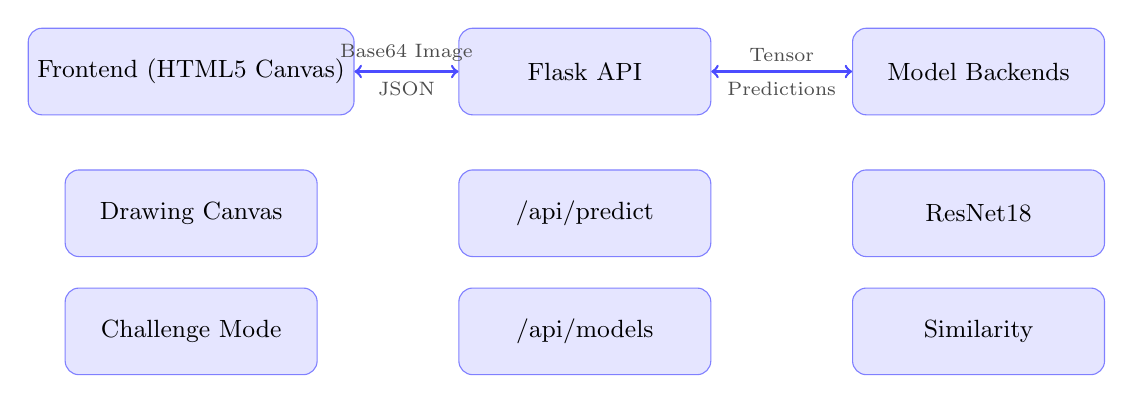
\begin{tikzpicture}[
    node distance=2.2cm,
    box/.style={rectangle, draw=blue!50, fill=blue!10, minimum width=3.2cm, minimum height=1.1cm, text centered, font=\small, rounded corners=5pt},
    arrow/.style={<->, thick, color=blue!70},
    label/.style={font=\scriptsize, color=black!70}
]

% Main components
\node[box] (frontend) {Frontend (HTML5 Canvas)};
\node[box, right of=frontend, node distance=5cm] (api) {Flask API};
\node[box, right of=api, node distance=5cm] (models) {Model Backends};

% Sub-components under Frontend
\node[box, below of=frontend, node distance=1.8cm] (canvas) {Drawing Canvas};
\node[box, below of=canvas, node distance=1.5cm] (challenge) {Challenge Mode};

% Sub-components under Flask API
\node[box, below of=api, node distance=1.8cm] (predict) {/api/predict};
\node[box, below of=predict, node distance=1.5cm] (models_api) {/api/models};

% Sub-components under Model Backends
\node[box, below of=models, node distance=1.8cm] (resnet) {ResNet18};
\node[box, below of=resnet, node distance=1.5cm] (similarity) {Similarity};

% Arrows between main components
\draw[arrow] (frontend) -- (api) node[midway, above, label] {Base64 Image};
\draw[arrow] (api) -- (frontend) node[midway, below, label] {JSON};
\draw[arrow] (api) -- (models) node[midway, above, label] {Tensor};
\draw[arrow] (models) -- (api) node[midway, below, label] {Predictions};

\end{tikzpicture}
\caption{Web Application Architecture}
\end{figure}

\subsubsection{Key Features}

\begin{enumerate}
    \item \textbf{Real-time Inference}: Predictions update every 400ms during drawing
    \item \textbf{Model Selection}: Switch between ResNet and Similarity models
    \item \textbf{Free Draw Mode}: Explore predictions without time pressure
    \item \textbf{Challenge Mode}: Gamified learning with scoring system
    \begin{itemize}
        \item \#1 prediction = 5 points
        \item \#2 prediction = 4 points
        \item \#3 prediction = 3 points
        \item \#4 prediction = 2 points
        \item \#5 prediction = 1 point
    \end{itemize}
    \item \textbf{Progress Tracking}: Streak counter, high score persistence
    \item \textbf{Drawing Tools}: Brush, eraser, undo/redo, adjustable brush size
    \item \textbf{Keyboard Shortcuts}: For efficient interaction
\end{enumerate}

\subsubsection{API Endpoints}

\begin{table}[H]
\centering
\caption{Flask API Endpoints}
\begin{tabular}{lll}
\toprule
\textbf{Endpoint} & \textbf{Method} & \textbf{Description} \\
\midrule
/api/models & GET & List available models \\
/api/model/\{key\} & POST & Set active model \\
/api/model/\{key\}/info & GET & Get model information \\
/api/predict & POST & Make prediction from canvas \\
/api/categories & GET & Get all category labels \\
/api/challenge & GET & Get random challenge word \\
\bottomrule
\end{tabular}
\end{table}

\subsection{Application Screenshots}

\begin{figure}[H]
    \centering
    \includegraphics[width=0.85\textwidth]{../proposal-dl/app_demo.png}
    \caption{Doodle Recognition Application - Main Interface showing real-time predictions}
    \label{fig:app_demo}
\end{figure}

\newpage

% ============================================================================
% 5. DISCUSSION & LIMITATIONS
% ============================================================================
\section{Discussion \& Limitations}

\subsection{Analysis of Results}

\subsubsection{ResNet18 Performance}

The ResNet18 model achieved 75.03\% top-1 accuracy, which is competitive with published results on the QuickDraw dataset. Key observations:

\begin{itemize}
    \item \textbf{Transfer Learning Effectiveness}: Pre-trained ImageNet features significantly improved convergence and final accuracy compared to training from scratch.
    
    \item \textbf{Two-Stage Training Benefits}: Freezing the backbone initially allowed the classifier to stabilize before fine-tuning, preventing catastrophic forgetting.
    
    \item \textbf{Top-3 Accuracy (90.70\%)}: The high top-3 accuracy suggests the model generally understands the drawing but may confuse similar categories (e.g., cat/tiger, apple/cherry).
    
    \item \textbf{Data Augmentation Impact}: Random rotation and affine transforms helped the model generalize to different drawing orientations and scales.
\end{itemize}

\subsubsection{Similarity Matching Baseline}

The OpenCV similarity approach (25-35\% accuracy) performed significantly worse than deep learning methods, highlighting:

\begin{itemize}
    \item \textbf{Limitation of Hand-crafted Features}: Template matching cannot capture the abstract variations in human drawings.
    
    \item \textbf{Computational Overhead}: Despite lower accuracy, similarity matching required more inference time due to comparisons with all templates.
    
    \item \textbf{Educational Value}: The approach serves as a useful baseline for understanding what deep learning learns.
\end{itemize}

\subsection{Challenges Encountered}

\begin{enumerate}
    \item \textbf{Class Imbalance}: Some categories had more varied drawings than others, affecting per-class accuracy.
    
    \item \textbf{Similar Categories}: Categories like ``cat'' and ``tiger'', or ``cup'' and ``mug'' caused confusion.
    
    \item \textbf{Abstract Drawings}: Highly abstract or incomplete drawings remained challenging.
    
    \item \textbf{Real-time Constraints}: Balancing model complexity with inference speed for smooth user experience.
    
    \item \textbf{Web Canvas Differences}: Canvas drawings have different characteristics than the QuickDraw training data.
\end{enumerate}

\subsection{Limitations}

\begin{enumerate}
    \item \textbf{Fixed Category Set}: The ResNet model cannot recognize categories outside the 340 trained classes without retraining.
    
    \item \textbf{Children's Drawing Gap}: Models trained on adult drawings may not generalize perfectly to children's drawings.
    
    \item \textbf{No Stroke Information}: Our bitmap-based approach loses the temporal stroke information that could improve recognition.
    
    \item \textbf{Single Language}: Current categories are English-only; extending to other languages requires localization.
    
    \item \textbf{No User Adaptation}: The model doesn't adapt to individual user's drawing style over time.
\end{enumerate}

\subsection{Trade-offs}

\begin{table}[H]
\centering
\caption{Model Selection Trade-offs}
\begin{tabular}{lll}
\toprule
\textbf{Criterion} & \textbf{ResNet18} & \textbf{OpenCV Similarity} \\
\midrule
Accuracy & High (75\%) & Moderate (25-35\%) \\
Model size & Large (44MB) & Small (templates only) \\
Inference speed & Fast (50ms) & Slower (~500ms) \\
Training data requirement & High & Low \\
Interpretability & Low & High \\
\bottomrule
\end{tabular}
\end{table}

\newpage

% ============================================================================
% 6. CONCLUSION & FUTURE WORK
% ============================================================================
\section{Conclusion \& Future Work}

\subsection{Conclusion}

This project successfully developed and deployed a comprehensive deep learning solution for real-time doodle recognition with educational applications. Our key achievements include:

\begin{enumerate}
    \item \textbf{Multiple Model Implementations}: We successfully implemented and compared two distinct approaches---ResNet18 transfer learning (75.03\% accuracy) and OpenCV similarity matching (25-35\% accuracy).
    
    \item \textbf{High Classification Performance}: The ResNet18 model achieved 90.70\% top-3 accuracy across 340 categories, demonstrating practical utility for educational applications where near-matches still provide learning value.
    
    \item \textbf{Real-time Web Application}: The Flask-based application provides smooth, real-time inference with predictions updating during drawing, creating an engaging user experience.
    
    \item \textbf{Gamification Integration}: The challenge mode with scoring mechanics transforms vocabulary learning into an interactive game, leveraging visual-motor learning principles.
    
    \item \textbf{Comprehensive Documentation}: All models are documented with training procedures, architecture details, and deployment instructions.
\end{enumerate}

The project demonstrates that deep learning can effectively recognize hand-drawn doodles in real-time, enabling new applications in educational technology. The combination of high accuracy, fast inference, and gamification creates a compelling tool for English vocabulary acquisition.

\subsection{Future Work}

Several directions could extend this project:

\begin{enumerate}
    \item \textbf{Stroke-based Recognition}: Incorporate temporal stroke information using RNNs or Transformers to improve accuracy on sequential drawing patterns.
    
    \item \textbf{Multi-lingual Support}: Add Indonesian translations and potentially other languages to reach broader audiences.
    
    \item \textbf{Adaptive Learning}: Implement user-specific model adaptation to improve recognition of individual drawing styles.
    
    \item \textbf{Mobile Deployment}: Port the application to mobile platforms (iOS/Android) for wider accessibility.
    
    \item \textbf{Classroom Integration}: Develop features for teachers to track student progress and customize vocabulary sets.
    
    \item \textbf{Ensemble Methods}: Combine ResNet and Similarity predictions for improved robustness.
    
    \item \textbf{Active Learning}: Collect user drawings to continuously improve model performance.
    
    \item \textbf{Children's Drawing Dataset}: Collect and train on drawings from Indonesian children to improve generalization.
\end{enumerate}

\newpage

% ============================================================================
% 7. REFERENCES
% ============================================================================
\section{References}

\begin{enumerate}[label={[\arabic*]}]
    \item K. He, X. Zhang, S. Ren, and J. Sun, ``Deep Residual Learning for Image Recognition,'' in \textit{Proceedings of the IEEE Conference on Computer Vision and Pattern Recognition (CVPR)}, 2016, pp. 770--778.
    
    \item D. Ha and D. Eck, ``A Neural Representation of Sketch Drawings,'' in \textit{International Conference on Learning Representations (ICLR)}, 2018.
    
    \item G. Koch, R. Zemel, and R. Salakhutdinov, ``Siamese Neural Networks for One-shot Image Recognition,'' in \textit{ICML Deep Learning Workshop}, 2015.
    
    \item O. Vinyals, C. Blundell, T. Lillicrap, K. Kavukcuoglu, and D. Wierstra, ``Matching Networks for One Shot Learning,'' in \textit{Advances in Neural Information Processing Systems (NeurIPS)}, 2016.
    
    \item Q. Yu, Y. Yang, F. Liu, Y.-Z. Song, T. Xiang, and T. M. Hospedales, ``Sketch-a-Net: A Deep Neural Network that Beats Humans,'' \textit{International Journal of Computer Vision}, vol. 122, no. 3, pp. 411--425, 2017.
    
    \item M. Tan and Q. Le, ``EfficientNet: Rethinking Model Scaling for Convolutional Neural Networks,'' in \textit{International Conference on Machine Learning (ICML)}, 2019.
    
    \item Google Creative Lab, ``Quick, Draw! Dataset,'' 2017. [Online]. Available: \url{https://github.com/googlecreativelab/quickdraw-dataset}
    
    \item A. Paszke et al., ``PyTorch: An Imperative Style, High-Performance Deep Learning Library,'' in \textit{Advances in Neural Information Processing Systems (NeurIPS)}, 2019.
    
    \item S. Deterding, D. Dixon, R. Khaled, and L. Nacke, ``From Game Design Elements to Gamefulness: Defining Gamification,'' in \textit{Proceedings of the 15th International Academic MindTrek Conference}, 2011, pp. 9--15.
\end{enumerate}

\newpage

% ============================================================================
% 8. APPENDIX
% ============================================================================
\section*{Appendix}
\addcontentsline{toc}{section}{Appendix}

\subsection*{A. Team Contribution Statement}

\begin{table}[H]
\centering
\caption{Team Member Contributions}
\begin{tabular}{|p{3cm}|p{10cm}|}
\hline
\textbf{Member} & \textbf{Contributions} \\
\hline
Valent Nathanael (2702343706) & 
\begin{itemize}[leftmargin=*, noitemsep, topsep=0pt]
    \item ResNet18 model architecture and training
    \item Web application backend (Flask API)
    \item Model integration and deployment
    \item Documentation and report writing
\end{itemize} \\
\hline
Joceline Araki (2702338334) & 
\begin{itemize}[leftmargin=*, noitemsep, topsep=0pt]
    \item Data preprocessing and augmentation
    \item Frontend UI/UX design
    \item Challenge mode gamification
\end{itemize} \\
\hline
Lauw, Samuel Lelono (2702348026) & 
\begin{itemize}[leftmargin=*, noitemsep, topsep=0pt]
    \item OpenCV similarity matching implementation
    \item Dataset preparation and exploration
    \item Model evaluation and comparison
    \item Testing and quality assurance
\end{itemize} \\
\hline
\end{tabular}
\end{table}

\textbf{Coordination Methods:}
\begin{itemize}
    \item Version control: Git/GitHub repository
    \item Communication: Weekly meetings and messaging
    \item Task management: GitHub Issues
    \item Code review: Pull request reviews
\end{itemize}

\subsection*{B. Sample Doodle Categories}

\begin{figure}[H]
    \centering
    \begin{minipage}{0.18\textwidth}
        \centering
        \includegraphics[width=\linewidth]{../proposal-dl/sample_1.png}
        \caption*{Apple}
    \end{minipage}\hfill
    \begin{minipage}{0.18\textwidth}
        \centering
        \includegraphics[width=\linewidth]{../proposal-dl/sample_2.png}
        \caption*{Banana}
    \end{minipage}\hfill
    \begin{minipage}{0.18\textwidth}
        \centering
        \includegraphics[width=\linewidth]{../proposal-dl/sample_3.png}
        \caption*{Tree}
    \end{minipage}\hfill
    \begin{minipage}{0.18\textwidth}
        \centering
        \includegraphics[width=\linewidth]{../proposal-dl/sample_4.png}
        \caption*{Car}
    \end{minipage}\hfill
    \begin{minipage}{0.18\textwidth}
        \centering
        \includegraphics[width=\linewidth]{../proposal-dl/sample_5.png}
        \caption*{Bus}
    \end{minipage}

    \vspace{1em}

    \begin{minipage}{0.18\textwidth}
        \centering
        \includegraphics[width=\linewidth]{../proposal-dl/sample_6.png}
        \caption*{Fish}
    \end{minipage}\hfill
    \begin{minipage}{0.18\textwidth}
        \centering
        \includegraphics[width=\linewidth]{../proposal-dl/sample_7.png}
        \caption*{Flower}
    \end{minipage}\hfill
    \begin{minipage}{0.18\textwidth}
        \centering
        \includegraphics[width=\linewidth]{../proposal-dl/sample_8.png}
        \caption*{House}
    \end{minipage}\hfill
    \begin{minipage}{0.18\textwidth}
        \centering
        \includegraphics[width=\linewidth]{../proposal-dl/sample_9.png}
        \caption*{Sun}
    \end{minipage}\hfill
    \begin{minipage}{0.18\textwidth}
        \centering
        \includegraphics[width=\linewidth]{../proposal-dl/sample_10.png}
        \caption*{Star}
    \end{minipage}
    \caption{Sample doodles from the QuickDraw dataset}
\end{figure}

\subsection*{C. Key Code Snippets}

\subsubsection*{ResNet18 Model Definition}

\begin{lstlisting}[style=python]
import torchvision.models as models
import torch.nn as nn

# Load pre-trained ResNet18
model = models.resnet18(weights='IMAGENET1K_V1')

# Replace classifier for 340 classes
num_features = model.fc.in_features
model.fc = nn.Sequential(
    nn.Dropout(0.5),
    nn.Linear(num_features, 512),
    nn.BatchNorm1d(512),
    nn.ReLU(inplace=True),
    nn.Dropout(0.3),
    nn.Linear(512, 340)
)
\end{lstlisting}

\subsubsection*{Flask Prediction Endpoint}

\begin{lstlisting}[style=python]
@app.route('/api/predict', methods=['POST'])
def predict():
    data = request.json
    image_data = data['image'].split(',')[1]
    image_bytes = base64.b64decode(image_data)
    
    # Convert to numpy array
    image = Image.open(io.BytesIO(image_bytes))
    img_array = np.array(image.convert('RGB'))
    
    # Get predictions from current model
    backend = model_backends[current_model_key]
    predictions = backend.predict(img_array, top_k=10)
    
    return jsonify({
        "predictions": [
            {"label": l, "confidence": c} 
            for l, c in predictions
        ]
    })
\end{lstlisting}

\subsection*{D. Project Repository}

The complete source code, trained models, and documentation are available at:

\begin{center}
\url{https://github.com/VennethN/doodle-recognition-comvis}
\end{center}

\textbf{Repository Structure:}
\begin{verbatim}
doodle-recognition/
+-- models/           # Trained model files
|   +-- resnet/       # ResNet18 model
|   +-- similarity/   # OpenCV classifier
+-- trainings/        # Jupyter notebooks
|   +-- doodle_recognition_model_resnet.ipynb
|   +-- doodle_similarity_matching.ipynb
+-- templates/        # HTML templates
+-- docs/             # Documentation
+-- web_app.py        # Flask application
+-- requirements.txt  # Dependencies
\end{verbatim}

\end{document}
